
% spellcheck: ok
% mikes: ok

\chapter[Seeing the Forest for the Trees]{Seeing the Forest for the
  Trees: Finding Important Attributes}{}{}
\label{ch:reduction}

\index{data analysis!dimensionality reduction|(}
\index{dimensionality reduction|(}
  
\Fint{What do you do when you don't know where to start? When you are
dealing with a data set that} offers no structure that would suggest an
angle of attack?

For example, I remember looking through a company's contracts with its
suppliers for a certain consumable. These contracts all differed in
regards to the supplier, the number of units ordered, the duration of
the contract and the lead time, the destination location that the
items were supposed to be shipped to, the actual shipping date, and
the procurement agent that had authorized the contract---and, of
course, the unit price. What I tried to figure out was which of these
quantities had the greatest influence on the unit price.

This kind of problem can be very difficult: there are so many
different variables, none of which seems, at first glance, to be
predominant. Furthermore, I have no assurance that the variables are
all independent; many of them may be expressing related information.
(In this case, the supplier and the shipping destination may be
related, since suppliers are chosen to be near the place where the
items are required.)

Because all variables arise on more or less equal footing, we can't
identify a few as the obvious ``control'' or independent variables and
then track the behavior of all the other variables in response to
these independent variables. We can try to look at all possible
pairings---for example, using graphical techniques such as
scatter-plot matrices (Chapter \ref{ch:multivariate})---but that may
not really reveal much either, particularly if the number of
variables is truly large. We need some form of computational guidance.

In this chapter, we will introduce a number of different techniques for
exactly this purpose. All of them help us select the most important
variables or \emph{features} from a multivariate data set in which all
variables appear to arise\vadjust{\pagebreak} on equal footing. In doing so, we
reduce the dimension of the data set from the original number of variables (or
features) to a smaller set, which (hopefully) captures most of the
``interesting'' behavior of the data. These methods are therefore also
known as \emph{feature selection} or \emph{dimensionality reduction}
techniques.

A word of warning: the material in this chapter is probably the most
advanced and least obvious in the whole book, both conceptually and
also with respect to actual implementations. In particular, the
following section (on principal component analysis) is very abstract,
and it may not make much sense if you haven't had some previous
exposure to matrices and linear algebra (including eigentheory). Other
sections are more accessible.

I include these techniques here nevertheless, because they are of
considerable practical importance but also to give you a sense of the
kinds of (more advanced) techniques that are available, and also as a
possible pointer for further study.


% ============================================================
\section{Principal Component Analysis}

\index{dimensionality reduction!principal component analysis (PCA)|(} 
\index{PCA (principal component analysis)|(} 

Principal component analysis (PCA) is the primary tool for
dimensionality reduction in multivariate problems. It is a
foundational technique that finds applications as part of many other,
more advanced procedures.
\subsection{Motivation}

\index{PCA (principal component analysis)!about|(}
 
To understand what PCA can do for us, let's consider a simple example.
Let's go back to the contract example given earlier and now assume
that there are only two variables for each contract: its lead time and
the number of units to be delivered. What can we say about them? Well,
we can draw histograms for each to understand the distribution of
values and to see whether there are ``typical'' values for either of
these quantities. The histograms (in the form of kernel density
estimates---see Chapter \ref{ch:univariate}) are shown in Figure
\ref{fig:pca1} and don't reveal anything of interest.

\begin{figure}
  \centerline{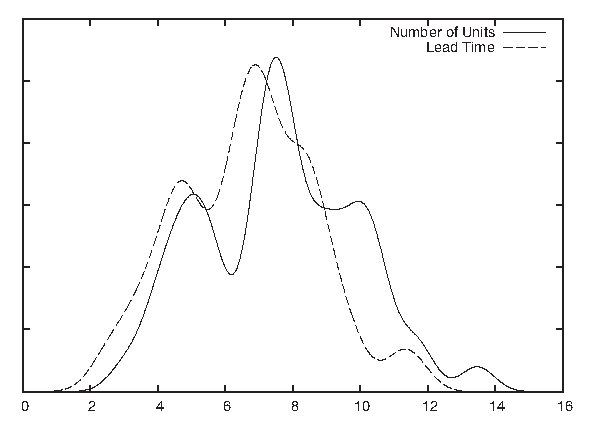
\includegraphics{img/pca1}}
  \caption{Contract data: distribution of points for the lead time and
    the number of units per order. The distributions do not reveal 
    anything in particular about the data.}
  \label{fig:pca1}
\end{figure}

Because there are only two variables in this case, we can also plot
one variable against the other in a scatter plot. The resulting graph
is shown in Figure \ref{fig:pca2} and is very revealing: the lead time
of the contract grows with its size. So far, so good.

\begin{figure}
  \centerline{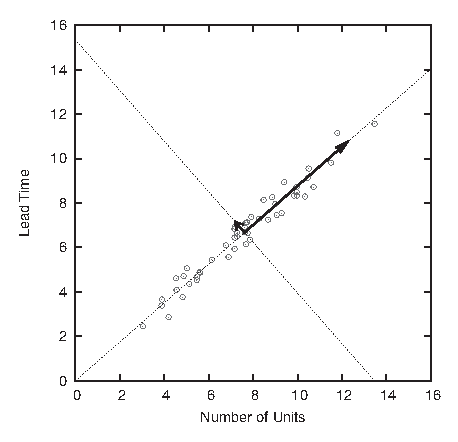
\includegraphics{img/pca2}}
  \caption{Contract data: individual contracts in a scatter plot
    spanned by the two original variables. All the points fall close
    to a straight line that is not parallel to either of the original
    coordinate axes.}
  \label{fig:pca2}
\end{figure}

But we can also look at Figure \ref{fig:pca2} in a different way.
Recall that the contract data depends on two variables (lead time and
number of items), so that we would expect the points to fill the
two-dimensional space spanned by the two axes (lead time and number of
items). But in reality, all the points fall very close to a straight
line. A straight line, however, is only one-dimensional, and this
means that we need only a \emph{single} variable to describe the
position of each point: the distance along the straight line.  In
other words, although it appears to depend on two variables, the
contract data \emph{mostly} depends on a single variable that lies
halfway between the original ones. In this sense, the data is of lower
dimensionality than it originally appeared.

Of course, the data still depends on two variables---as it did
originally.  But most of the \emph{variation} in the data occurs along
only one direction. If we were to measure the data only along this
direction, we would still capture most of what is ``interesting''
about the data.  In Figure \ref{fig:pca3}, we see another kernel
density estimate of the same data, but this time not taken along the
original variables but\vadjust{\pagebreak} instead showing the distribution of data
points along the two ``new'' directions indicated by the arrows in the
scatter plot of Figure \ref{fig:pca2}. In contrast to the variation
occurring along the ``long'' component, the ``short'' component is
basically irrelevant.

\begin{figure}
  \centerline{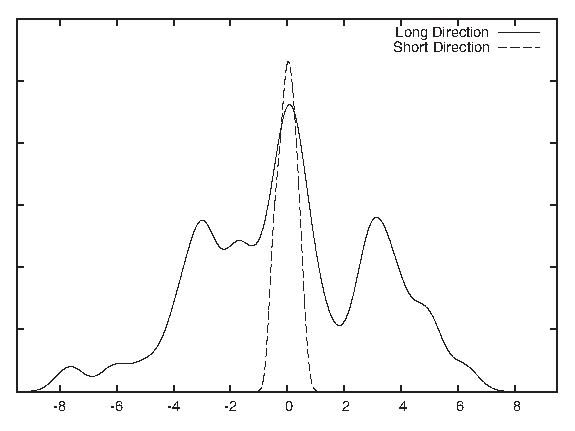
\includegraphics{img/pca3}}
  \caption{Contract data: distribution of points along the principal
    directions. Most of the variation is along the ``long'' direction,
    whereas there is almost no variation perpendicular to it. (The
    vertical scales have been adjusted to make the curves
    comparable.)}
  \label{fig:pca3}
\end{figure}

For this simple example, which had only two variables to begin with,
it was easy enough to find the lower-dimensional representation just
by looking at it. But that won't work when there are significantly
more than two variables involved. If there aren't too many variables,
then we can generate a scatter-plot matrix (see Chapter
\ref{ch:multivariate}) containing all possible pairs of variables, but
even this becomes impractical once there are more than seven or eight
variables.  Moreover, scatter-plot matrices can never show us more
than the combination of any two of the original variables. What if the
data in a three-dimensional problem falls onto a straight line that
runs along the \emph{space} diagonal of the original three-dimensional
data cube? We will not find this by plotting the data against any
(two-dimensional!) pair of the original variables.

Fortunately, there is a calculational scheme that---given a set of
points---will give us the principal directions (in essence, the arrows
in Figure \ref{fig:pca2}) as a combination of the original variables.
That is the topic of the next section.

\index{PCA (principal component analysis)!about|)}

\subsection{Optional: Theory}

\index{PCA (principal component analysis)!theory|(}
 
We can make progress by using a technique that works for many
multi-dimensional problems. If we can summarize the available
information regarding the multi-dimensional system in \emph{matrix
  form}, then we can invoke\vadjust{\pagebreak} a large and powerful body of results
from linear algebra to transform this matrix into a form that reveals any
underlying structure (such as the structure visible in Figure
\ref{fig:pca2}).

In what follows, I will often appeal to the two-dimensional example of
Figure \ref{fig:pca2}, but the real purpose here is to develop a
procedure that will be applicable to any number of dimensions. These
techniques become necessary when the number of dimensions exceeds two
or three so that simple visualizations like the ones discussed so far
will no longer work.

To express what we know about the system, we first need to ask
ourselves how best to summarize the way any two variables relate to
each other. Looking at Figure \ref{fig:pca2}, the \emph{correlation
  coefficient} \index{correlation coefficient!PCA} suggests itself.  In Chapter \ref{ch:clustering}, we
introduced the correlation coefficient as a measure for the similarity
between two multi-dimensional \emph{data points} $x$ and $y$. Here, we
use the same concept to express the similarity between two
\emph{dimensions} in a multivariate data set. Let $x$ and $y$ be two
different dimensions (``variables'') in such a data set, then the
correlation coefficient is defined by:
%
\[ 
\operatorname{corr}(x,y) 
  = \frac{1}{N}
    \frac{ \sum_i ( x_i - \bar{x} ) ( y_i - \bar{y} ) } 
         { \sigma(x) \sigma(y) }
\]
%
where the sum is over all data points, $\bar{x}$ and $\bar{y}$ are the
means of the $x_i$ and the $y_i$, respectively, and $\sigma(x) = \sqrt{
  \frac{1}{N} \sum_i (x_i - \bar{x})^2 }$ is the standard deviation of
$x$ (and equivalently for $y$). The denominator in the expression of
the correlation coefficient amounts to a rescaling of the values of
both variables to a standard interval. If that is not what we want,
then we can instead use the \emph{covariance} between the $x_i$ and
the $y_i$:
%
\[ 
\operatorname{cov}(x,y)
   = \frac{1}{N} \sum_i^N ( x_i - \bar{x} ) ( y_i - \bar{y} ) 
\]
%

All of these quantities can be defined for \emph{any} two variables
(just supply values for, say $x_i$ and $z_i$). For a $p$-dimensional
problem, we can find all the $p(p-1)/2$ different combinations
(remember that these coefficients are symmetric:
$\operatorname{cov}(x,y) = \operatorname{cov}(y,x)$).

It is now convenient to group the values in a matrix, which is
typically called $\Sigma$ (not to be confused with the summation
sign!)
%
\[
\Sigma = 
\begin{pmatrix}
\operatorname{cov}(x,x) & \operatorname{cov}(x,y) & \dots \\
\operatorname{cov}(y,x) & \operatorname{cov}(y,y) & \\
\vdots &  & \ddots 
\end{pmatrix}
\]
%
and similarly for the correlation matrix. Because the covariance (or
correlation) itself is symmetric under an interchange of its
arguments, the matrix $\Sigma$ is also symmetric (so that it equals
its transpose).

We can now invoke an extremely important result from linear algebra,
known as the \emph{spectral decomposition theorem}, \index{spectral decomposition theorem} as follows.
\emph{
For any real, symmetric $N \times N$ matrix $A$, there exists an 
orthogonal matrix $U$ such that:
%
\[
B =
\begin{pmatrix}
\lambda_1 &           &        &           \\
          & \lambda_2 &        &           \\
          &           & \ddots &           \\
          &           &        & \lambda_N
\end{pmatrix}
= U^{-1} A U
\]
is a diagonal matrix.} 

% http://mathworld.wolfram.com/EigenDecompositionTheorem.html

Let's explain some of the terminology. A matrix is \emph{diagonal} if
its only nonzero entries are along the main diagonal from the top left
to the bottom right. A matrix is \emph{orthogonal} if its transpose
equals its inverse: $U^T = U^{-1}$ or $U^T U = U U^T = 1$.

The entries $\lambda_i$ in the diagonal matrix are called the
\emph{eigenvalues} of matrix $A$, and the column vectors of $U$ are the
\emph{eigenvectors}.\index{eigenvectors}\index{vectors!eigenvectors} The
spectral theorem also implies that all eigenvectors are mutually
orthogonal. Finally, the $i$th column vector in $U$ is the eigenvector
``associated'' with the eigenvalue
$\lambda_i$; each eigenvalue has an associated eigenvector.

What does all of this mean?  In a nutshell, it means that we can
perform a change of variables that turns any symmetric matrix $A$ into
a diagonal matrix $B$.  Although it may not be obvious, the matrix $B$
contains the same information as $A$---it's just packaged differently.

The change of variables required for this transformation consists of a
\emph{rotation} of the original coordinate system into a new
coordinate system in which the correlation matrix has a particularly
convenient (diagonal) shape. (Notice how in Figure \ref{fig:pca2}, the
new directions are rotated with respect to the original horizontal and
vertical axes.)

When expressed in the original coordinate system (\ie, the original
variables that the problem was initially expressed in), the matrix
$\Sigma$ is a complicated object with off-diagonal entries that are
nonzero.  However, the eigenvectors span a new coordinate system that
is rotated with respect to the old one. In this new coordinate system,
the matrix takes on a simple, diagonal form in which all entries that
are not on the diagonal vanish. The arrows in Figure \ref{fig:pca2}
show the directions of the new coordinate axes, and the histogram in
Figure \ref{fig:pca3} measures the distribution of points along these
new directions.

The purpose of performing a matrix diagonalization is to find the
directions of this new coordinate system, which is more suitable for
describing the data than was the original coordinate system.

Because the new coordinate system is merely rotated relative to the
original one, we can express its coordinate axes as linear
combinations of the original ones. In Figure \ref{fig:pca2}, for
instance, to make a step in the new direction (along the diagonal), you
take a step along the (old) $x$ axis,\vadjust{\pagebreak} followed by a step along the
(old) $y$ axis. We can therefore express the new direction (call it
$\hat{x}$) in terms of the old ones: $\hat{x} = (x + y)/\sqrt{2}$ (the
factor $\sqrt{2}$ is just a normalization factor).

\index{PCA (principal component analysis)!theory|)}

\subsection{Interpretation}

\index{PCA (principal component analysis)!interpretation}
 
The spectral decomposition theorem applies to \emph{any} symmetric
matrix. For any such matrix, we can find a new coordinate system, in
which the matrix is diagonal. But the \emph{interpretation} of the
results (what do the eigenvalues and eigenvectors mean?) depends on
the specific application.  In our case, we apply the spectral theorem
to the covariance or correlation matrix of a set of points, and the
results of the decomposition will give us the \emph{principal axes of
  the distribution of points} (hence the name of the technique).

Look again at Figure \ref{fig:pca2}. Points are distributed in a
region shaped like an extremely stretched ellipse. If we calculate the
eigenvalues and eigenvectors of the correlation matrix of this point
distribution, we find that the eigen\emph{vectors}\index{eigenvectors}\index{vectors!eigenvectors} 
lie in the directions of the principal axes
of the ellipse while the eigen\emph{values} give the relative length of
the corresponding principal axes.

Put another way, the eigenvalues point along the directions of
greatest variance: the data is most stretched out if we measure it
along the principal directions. Moreover, the eigenvalue corresponding
to each eigenvector is a measure of the width of the distribution along
this direction. 

(In fact, the eigenvalue is the square of the standard deviation along
that direction; remember that the diagonal entries of the covariance
matrix $\Sigma$ are $\sigma^2(x) = \sum_i (x_i - \bar{x})^2$.  Once we
diagonalize $\Sigma$, the entries along the diagonal---that is, the
eigenvalues---are the variances along the ``new'' directions.)

You should also observe that the variables measured along the
principal directions are uncorrelated with each other. (By
construction, their correlation matrix is diagonal, which means that
the correlation between any two different variables is zero.)

This, then, is what the principal component analysis does for us: if
the data points are distributed as a globular cloud in the space
spanned by all the original variables (which may be more than two!),
then the eigenvectors will give us the \emph{directions} of the
principal axes of the ellipsoidal cloud of data points and the
eigenvalues will give us the \emph{length} of the cloud along each of
these directions. The eigenvectors and eigenvalues therefore describe
the shape of the point distribution. This becomes especially useful if
the data set has more than just two dimensions, so that a simple plot
(as in Figure \ref{fig:pca2}) is no longer feasible.  (There are
special varieties of PCA, such as ``Kernel PCA'' or ``ISOMAP,'' that
work even with point distributions that do not form globular
ellipsoids but have more complicated, contorted shapes.)

The description of the shape of the point distribution provided by the
PCA is already helpful. But it gets even\vadjust{\pagebreak} better, because we may
suspect that not all of the original variables are really needed. Some
of them may be redundant (expressing more or less the same thing), and
others may be irrelevant (carrying little information).

An indication that variables may be redundant (\ie, express the ``same
thing'') is that they are correlated. (That's pretty much the
definition of correlation: knowing that if we change one variable,
then there will be a corresponding change in the other.)  The PCA uses
the information contained in the mutual correlations between variables
to identify those that are redundant. By construction, the principal
coordinates are \emph{uncorrelated} (\ie, not redundant), which means
that the information contained in the original (redundant) set of
variables has been concentrated in only a few of the new variables
while the remaining variables have become irrelevant.  The irrelevant
variables are those corresponding to small eigenvalues: the point
distribution will have only little spread in the corresponding
directions (which means that these variables are almost constants and
can therefore be ignored).

The price we have to pay for the reduction in dimensions is that the
new directions will not, in general, map neatly to the original
variables. Instead, the new directions will correspond to
\emph{combinations} of the original variables.

There is an important consequence of the preceding discussion: the
principal component analysis works with the correlation between
variables. If the original variables are uncorrelated, then there is
no point in carrying out a PCA! For instance, if the data points in
Figure \ref{fig:pca2} had shown no structure but had filled the
entire two-dimensional parameter space randomly, then we would not
have been able to simplify the problem by reducing it to a
one-dimensional one consisting of the new direction along the main
diagonal.

% For the data set shown in figure \ref{fig:pca2}, it is an easy
% excercise to work out the eigenvectors and eigenvalues. The direction
% of the eigenvectors is indicated in the figure, and the two
% eigenvalues are:
% 
% \begin{align*}
% \lambda_1 & = 3.3862 \\
% \lambda_2 & = 0.1307
% \end{align*}


\subsection{Computation}

\index{PCA (principal component analysis)!computation}
 
The theory just described would be of only limited interest if there
weren't practical algorithms for calculating both eigenvalues and
eigenvectors.  These calculations are always numerical.  You may have
encountered algebraic methods matrix diagonalization methods in
school, but they are impractical for matrices larger than $2 \times 2$
and infeasible for matrices larger than about $4 \times 4$.

However, there are several elegant \emph{numerical} algorithms to
invert and diagonalize matrices, and they tend to form the
foundational part of any numerical library. They are not trivial to
understand, and developing high-quality implementations (that avoid,
say round-off error) is a specialized skill. There are no good
reasons to write your own, so you should always use an established
library. (Every numerical library or package will include the required
functionality.)

Matrix operations\index{matrix operations}\index{performance!matrix
operations and other computational applications} are relatively
expensive, and run time performance can be a serious concern for large
matrices. Matrix operations tend to be of $\mathcal{O}(N^3)$ complexity,
which means that doubling the size\vadjust{\pagebreak} of the matrix will
increase the time to perform an operation by a factor of $2^3 = 8$. In
other words, doubling the problem size will result in nearly a
\emph{tenfold} increase in runtime! This is not an issue for small
matrices (up to $100 \times 100$ or so), but you will hit a brick wall
at a certain size (somewhere between $\text{5,000}
\times \text{5,000}$ and $\text{50,000} \times \text{50,000}$). Such
large matrices do occur in practice but usually not in the context of
the topic of this chapter.  For even larger matrices there are
alternative algorithms---\break which, however, calculate only the most
important of the eigenvalues and eigenvectors.

I will not go into details about different algorithms, but I want to
mention one explicitly because it is of particular importance in this
context.  If you read about principal component analysis (PCA),
then you will likely encounter the term \emph{singular value
  decomposition} (SVD);\index{SVD (singular value decomposition)}\index{singular value decomposition (SVD)} in fact, many books treat PCA and SVD as
equivalent expressions for the same thing. That is not correct; they
are really quite different. PCA is the application of spectral methods
to covariance or correlation matrices; it is a conceptual technique,
not an algorithm. In contrast, the SVD is a specific algorithm that
can be applied to many different problems one of which is the PCA.

The reason that the SVD features so prominently in discussions of the
PCA is that the SVD combines two required steps into one.  In our
discussion of the PCA, we assumed that you first calculate the
covariance or correlation matrix explicitly from the set of data
points and then diagonalize it. The SVD performs these two steps in
one fell swoop: you pass the set of data points directly to the SVD,
and it calculates the eigenvalues and eigenvectors of the correlation
matrix directly from those data points. 

The SVD is a very interesting and versatile algorithm, which is
unfortunately rarely included in introductory classes on linear
algebra.

\subsection{Practical Points}

\index{PCA (principal component analysis)!issues}
 
As you can see, principal component analysis is an involved
technique---although with the appropriate tools it becomes almost
ridiculously easy to perform (see the Workshop in this chapter). But
convenient implementations don't make the conceptual difficulties go
away or ensure that the method is applied appropriately.

First, I'd like to emphasize that the mathematical operations
underlying principal component analysis (namely, the diagonalization
of a matrix) are very general: they consist of a set of formal
transformations that apply to \emph{any} symmetric matrix.
(Transformations of this sort are used for many different purposes
in literally all fields of science and engineering.)

In particular, there is nothing specific to data analysis about these
techniques. The PCA thus does not involve any of the concepts that we
usually deal with in statistics or analysis: there is no mention of
populations, samples, distributions, or models. Instead, principal
component analysis is a set of formal transformations, which are
applied to the covariance matrix of a data set. As such, it can be
either \emph{exploratory} or \emph{preparatory}.

As an exploratory technique, we may inspect its results (the
eigenvalues and eigenvectors) for anything that helps us develop an
understanding of the data set. For example, we may look at the
contributions to the first few principal components to see whether we
can find an intuitive interpretation of them (we will see an example
of this in the Workshop section).  Biplots (discussed in the following
section) are a graphical technique that can be useful in this context.

But we should keep in mind that this kind of investigation is
exploratory in nature: there is no guarantee that the results of a
principal component analysis will turn up anything useful. In
particular, we should not expect the principal components to have an
intuitive interpretation in general.

On the other hand, PCA may also be used as a preparatory technique.
Keep in mind that, by construction, the principal components are
uncorrelated. We can therefore transform any multivariate data set into
an equivalent form, in which all variables are mutually independent,
before performing any subsequent analysis.  Identifying a subset of
principal components that captures most of the variability in the data
set---for the purpose of reducing the dimensionality of the problem,
as we discussed earlier---is another preparatory use of principal
component analysis.

As a preparatory technique, principal component analysis is always
applicable but may not always be useful. For instance, if the original
variables are already uncorrelated, then the PCA cannot do anything
for us. Similarly, if none of the eigenvalues are significantly
smaller (so that their corresponding principal components can be
dropped), then again we gain nothing from the PCA.

Finally, let me reiterate that PCA is just a mathematical
transformation that can be applied to any symmetric matrix. This means
that its results are not uniquely determined by the data set but
instead are sensitive to the way the inputs are prepared. In
particular, the results of a PCA depend on the actual \emph{numerical
  values} of the data points and therefore on the \emph{units} in
which the measurements have been recorded. If the numerical values for
one of the original variables are consistently larger than the values
of the other variables, then the variable with the large values will
unduly dominate the spectrum of eigenvalues. (We will see an example
of this problem in the Workshop.) To avoid this kind of problem, all
variables should be of comparable scale. A systematic way to achieve
this is to work with the correlation matrix (in which all entries are
normalized by their autocorrelation) instead of the covariance matrix.

\subsection{Biplots}

\index{PCA (principal component analysis)!biplots}
\index{biplots, PCA}
  
Biplots are an interesting way to visualize the results of a principal
component analysis.  In a biplot, we plot the data points in a
coordinate system spanned by the first two principal components (\ie,
those two of the \emph{new} variables corresponding to the largest
eigenvalues). In addition, we also\vadjust{\pagebreak} plot a representation of the
\emph{original} variables but now projected into the space of the new
variables. The data points are represented by symbols, whereas the
directions of the original variables are represented by arrows. (See
Figure \ref{fig:biplot} in the Workshop section.)

In a biplot, we can immediately see the distribution of points when
represented through the new variables (and can also look for clusters,
outliers, or other interesting features). Moreover, we can see how the
original variables relate to the first two principal components and to
each other: if any of the original variables are approximately aligned
with the horizontal (or vertical) axis, then they are approximately
aligned with the first (or second) principal component (because in a
biplot, the horizonal and vertical axes coincide with the first and
second principal components). We can thus see which of the original
variables contribute strongly to the first principal components, which
might help us develop an intuitive interpretation for those
components.  Furthermore, any of the original variables that are
roughly redundant will show up as more or less parallel to each other
in a biplot---which can likewise help us identify such combinations of
variables in the original problem.

Biplots may or may not be helpful. There is a whole complicated set of
techniques for interpreting biplots and reading off various quantities
from them, but these techniques seem rarely used, and I have not found
them to be very practical.  If I do a PCA, I will routinely also draw
a biplot: if it tells me something worthwhile, that's great; but if
not, then I'm not going to spend much time on it.

\index{dimensionality reduction!principal component analysis (PCA)|)} 
\index{PCA (principal component analysis)|)} 

% \subsection{PCA Variants}
% 
% kPCA
% ISOMAP (using ``Geodetic'' distances measured ALONG the manifold)
% ICA?

% ============================================================
\section{Visual Techniques}

\index{dimensionality reduction!visual techniques} 

Principal component analysis is a rigorous prescription, and example
of a ``data-centric'' technique: it transforms the original data in a
precisely prescribed way, without ambiguity and without making further
assumptions. The results are an expression of properties of the data
set. It is up to us to interpret them, but the results are true
regardless of whether we find them useful or not.

In contrast, the methods described in this section are convenience
methods that attempt to make multi-dimensional data sets more
``palatable'' for human consumption. These methods do not calculate
any rigorous properties inherent in the data set; instead, they try to
transform the data in such a way that it can be plotted while at the
same time trying to be as faithful to the data as possible.

We will not discuss any of these methods in depth, since personally, I
do not find them worth the effort: on the one hand, they are (merely)
exploratory in nature; on the other hand, they require rather heavy
numerical computations and some nontrivial theory.  Their primary
results are projections (\ie, graphs) of data sets, which can be
difficult to interpret if the number of data points or their
dimensionality becomes large---which is exactly when I expect a
computationally intensive method to be helpful!  Nevertheless,\vadjust{\pagebreak} there
are situations where you might find these methods useful, and they do
provide some interesting concepts for how to \emph{think} about data.
This last reason is the most important to me, which is why this
section emphasizes concepts while skipping most of the technical
details.
 
% The next para is a little orphaned...

The methods described in this section try to calculate specific
``views'' or projections of the data into a lower number of
dimensions.  Instead of selecting a specific projection, we can also
try to display many of them in sequence, leaving it to the human
observer to choose those that are ``interesting.'' That is the method
we introduced in Chapter \ref{ch:multivariate}, when we discussed
Grand Tours and Projection Pursuits---they provide yet another
approach to the problem of dimensionality reduction for multivariate
data sets.
 

\subsection{Multidimensional Scaling}

\index{MDS (multidimensional scaling)} 
\index{multidimensional scaling (MDS)} 

Given a set of data points (\ie, the \emph{coordinates} of each data
point), we can easily find the distance between any pair of points
(see Chapter \ref{ch:clustering} for a discussion of distance
measures). Multidimensional scaling (MDS) attempts to answer the
opposite question: given a distance matrix, can we recover the
explicit coordinates of the points?

This question has a certain intellectual appeal in its own right, but
of course, it is relevant in situations where our information about a
certain system is limited to the differences between data points.  For
example, in usability studies or surveys we may ask respondents to
list which of a set of cars (or whiskeys, or pop singers) they find
the most or the least alike; in fact, the entire method was first
developed for use in psychological studies. The question is: given
such a matrix of relative preferences or distances, can we come up
with a set of absolute positions for each entry?

First, we must choose the desired number of dimensions of our points.
The dimension $D=2$ is used often, so that the results can be plotted
easily, but other values for $D$ are also possible.

If the distance measure is Euclidean---that is, if the distance
between two points is given by:
%
\[
d( x, y ) = \sqrt{ \sum_i^D ( x_i - y_i )^2 }
\]
% 
where the sum is running over all dimensions---then it turns out that
we can invert this relationship explicitly and find expressions for
the coordinates in terms of the distances. (The only additional
assumption we need to make is that the center of mass of the entire
data set lies at the origin, but this amounts to no more than an
arbitrary translation of all points.) This technique is known as
\emph{classical} or \emph{metric scaling}.

The situation is more complicated if we cannot assume that the
distance measure is Euclidean. Now we can no longer invert the
relationship exactly and must resort instead to iterative
approximation schemes.\vadjust{\pagebreak} Because the resulting coordinates may not
replicate the original distances exactly, we include an additional
constraint: the distance matrix calculated from the new positions must
obey the same rank order as the original distance matrix: if the
original distances between any three points obeyed the relationship
$d(x,y) < d(x,z)$, then the calculated coordinates of the three points
must satisfy this also.  For this reason, this version of
multidimensional scaling is known as \emph{ordinal scaling}.

The basic algorithm makes an initial guess for the coordinates and
calculates a distance matrix based on the guessed coordinates.  The
coordinates are then changed iteratively to minimize the discrepancy
(known as the ``stress'') between the new distance matrix and the
original one.

Both versions of multidimensional scaling lead to a set of coordinates
in the desired number of dimensions (usually two), which we can use to
plot the data points in a form of scatter plot. We can then inspect
this plot for clusters, outliers, or other features.

\vspace*{-6pt}
\subsection{Network Graphs}

\index{network graphs}
 
In passing, I'd like to mention \emph{force-based algorithms}
\index{force-based algorithms} for drawing network graphs because they
are similar in spirit to multidimensional scaling.

Imagine we have a network consisting of nodes, some of which are
connected by vertices (or edges), and we would like to find a way to
plot this network in a way that is ``attractive'' or ``pleasing.''
One approach is to treat the edges as springs, in such a way that each
spring has a preferred extension and exerts an opposing force---in the
direction of the spring---if compressed or extended beyond its
preferred length. We can now try to find a configuration (\ie, a set
of coordinates for all nodes) that will minimize the overall tension
of the springs.

There are basically two ways we can go about this. We can write down
the the total energy due to the distorted springs and then minimize it
with respect to the node coordinates using a numerical minimization
algorithm. Alternatively, we can ``simulate'' the system by
initializing all nodes with random coordinates and then iteratively
moving each node in response to the spring forces acting on it. For
smaller networks, we can update all nodes at the same time; for very
large networks, we may randomly choose a single node at each iteration
step for update and continue until the configuration no longer
changes. It is easy to see how this basic algorithm can be extended
to include richer situations---for instance, edges carrying different
weights.

Note that this algorithm makes no guarantees regarding the distances
that are maintained between the nodes in the final configuration. It
is purely a visualization technique.

\vspace*{-6pt}
% ============================================================
\section{Kohonen Maps}

\index{dimensionality reduction!Kohonen maps|(} 
\index{Kohonen maps|(} 

Self-organizing maps (SOMs),\index{SOMs (self-organizing maps)}\index{self-organizing maps (SOMs)} often called Kohonen maps after their
inventor, are different from the techniques discussed so far. In both
principal component analysis and multidimensional scaling, we
attempted\vadjust{\pagebreak} to find a new, more favorable
arrangement of points by moving them about in a continuous fashion.
When constructing a Kohonen map, however, we map the original data
points to cells in a \emph{lattice}. The presence of a lattice forces a
fixed topology on the system; in particular, each point in a lattice
has a fixed set of neighbors. (This property is typically and
confusingly called ``ordering'' in most of the literature on Kohonen
maps.)

The basic process of constructing a Kohonen map works as follows. We
start with a set of $k$ data points in $p$ dimensions, so that each
data point consists of a tuple of $p$ numeric values.  (I
intentionally avoid the word ``vector'' here because there is no
requirement that the data points must satisfy the ``mixable'' property
characteristic of vectors---see Appendix \ref{app:data} and Chapter
\ref{ch:clustering}.)

Next we prepare a lattice. For simplicity, we consider a
two-dimensional square lattice consisting of $n \times m$ cells.  Each
cell contains a $p$-dimensional tuple, similar to a data point, which
is called the \emph{reference tuple}. We initialize this tuple with
random values. In other words, our lattice consists of a collection of
random data points, arranged on a regular grid.

Now we perform the following iteration. For each data point, we find
that cell in the lattice with the smallest distance between its
contained $p$-tuple and the data point; then we assign the data point
to this cell. Note that multiple data points can be assigned to the
same cell if necessary.

Once all the data points have been assigned to cells in the lattice,
we update the $p$-tuples of all cells based on the values of the data
points assigned to the cell itself and to its neighboring cells. In
other words, we use the data points assigned to each cell, as well as
those assigned to the cell's neighbors, to compute a new tuple for the
cell.

When all lattice points have been updated, we restart the iteration
and begin assigning data points to cells again (after erasing the
previous assignments). We stop the iteration if the assignments no
longer change or if the differences between the original cell values
and their updates are sufficiently small.

This is the basic algorithm for the construction of a Kohonen map.  It
has certain similarities with the $k$-means algorithm discussed in
Chapter \ref{ch:clustering}. Both are iterative procedures in which
data points are assigned to cells or clusters, and the cell or cluster
is updated based on the points assigned to it.  However, two features
are specific to Kohonen maps:

\begin{itemize}
\item Each data point is mapped to a cell in the lattice, and this
  implies that each data point is placed in a specific neighborhood of
  other data points (which have been mapped to neighboring cells).
\item Because the updating step for each cell relies not only on the
  current cell but also on neighboring cells, the resulting map will
  show a ``smooth'' change of values: changes are averaged or
  ``smeared out'' over all cells in the neighborhood. Viewed the other
  way around, this implies that points that are similar to each other
  will map to lattice cells that are in close proximity to each other.
\end{itemize}

Although the basic algorithm seems fairly simple, we still need to
decide on a number of technical details if we want to develop a
concrete implementation. Most importantly, we still need to give a
specific prescription for how the reference tuples will be updated by
the data points assigned to the current cell and its neighborhood.

In principle, it would be possible to recalculate the values for the
reference tuple from scratch every time by forming a componentwise
average of all data points assigned to the cell. In practice, this may
lead to instability during iteration, and therefore it is usually
recommended to perform an incremental update of the reference value
instead, based on the difference between the current value of the
reference tuple and the assigned data points. If $y_i(t)$ is the value
of the reference tuple at position $i$ and at iteration $t$, then we
can write its value at the next iteration step $t+1$ as:
%
\[
y_i(t+1) = y_i(t) + \sum_k h(i, j; t) \paren{ x_k(j;t) - y_i(t) }
\]
%
where $x_k(j;t)$ is the data point $k$ which has been assigned to
lattice point $j$ at iteration step $t$ and where the sum runs over
all data points. The weight function $h(i, j; t)$ is now chosen to be
a decreasing function of the distance between the lattice cells $i$
and $j$, and it is also made to shrink in value as the iteration
progresses.  A typical choice is a Gaussian:
%
\[
h(i, j; t) = \alpha(t) \exp \paren{ - \frac{ d_{ij} }{2 \sigma(t) } }^2
\]
%
where $d_{ij}$ is the Euclidean distance between lattice points $i$
and $j$ and where $\alpha(t)$ and $\sigma(t)$ are decreasing functions
of $t$.  Choices other than the Gaussian are also possible---for
instance, we may choose a step function to delimit the effective
neighborhood.

Even with these definitions, we still need to decide on further
details:

\begin{itemize}
\item What is the topology of the lattice? Square lattices (like
  quad-ruled paper) are convenient but strongly single out two
  specific directions. Hexagonal lattices (like a honeycomb) are more
  isotropic. We also need to fix the boundary conditions. Do cells at
  the edge of the lattice have fewer neighbors than cells in the
  middle of the lattice, or do we wrap the lattice around and connect
  the opposite edges to form periodic boundary conditions?
\item What is the size of the lattice? Obviously, the number of cells
  in the lattice should be smaller than the number of data points
  (otherwise, we end up with unoccupied cells). But how much smaller?
  Is there a preferred ratio between data points and lattice cells?
  Also, should the overall lattice be square ($n \times n$) or
  rectangular ($n \times m$)? In principle, we can even consider
  lattices of different shape---triangular, for example, or circular.
  However, if we choose a lattice of higher symmetry (square or
  circular), then the \emph{orientation} of the final result within
  the lattice is not fixed; for this reason, it has been suggested
  that the lattice should always be oblongated (\eg, rectangular
  rather than square).
\item We need to choose a distance or similarity measure for measuring
  the distance between data points and reference tuples.
\item We still need to fix the numerical range of $\alpha(t)$ and
  $\sigma(t)$ and define their behavior as functions of $t$.
\end{itemize}

In addition, there are many opportunities for low-level tuning, in
particular with regard to performance and convergence. For example, we
may find it beneficial to initialize the lattice points with values
other than random numbers.

Finally, we may ask what we can actually do with the resulting lattice
of converged reference tuples. Here are some ideas.

\begin{itemize}
\item We can use the lattice to form a smooth, ``heat map''
  visualization of the original data set. Because cells in the lattice
  are closely packed, a Kohonen map interpolates smoothly between
  different points. This is in contrast to the result from either PCA
  or MDS, which yield only individual, scattered points.
\item One problem when plotting a Kohonen map is deciding which
  feature to show. If the original data set was $p$-dimensional,
  you may have to plot $p$ different graphs to see the distribution
  of all features.
\item The situation is more favorable if one of the features of
  interest is categorical and has only a few possible values. In this
  case, you can plot the labels on the graph and study their
  relationships (which labels are close to each other, and so on). In
  this situation, it is also possible to use a ``trained'' Kohonen map
  to classify new data points or data points with missing data.
\item If the number of cells in the lattice was chosen much smaller
  than the number of original data points, then you can try mapping
  the reference tuples \emph{back} into the original data space---for
  example, to use them as \emph{prototypes} for clustering purposes.
\end{itemize}

Kohonen maps are an interesting technique that occupy a space
between clustering and dimensionality reduction. Kohonen maps group
similar points together like a clustering algorithm, but they also
generate a low-dimensional representation of all data points by
mapping all points to a low-dimensional lattice. The entire concept is
very ad hoc and heuristic; there is little rigorous theory, and thus
there is little guidance on the choice of specific details.
Nonetheless, the hands-on, intuitive nature of Kohonen maps lends
itself to exploration and experimentation in a way that a more
rigorous (but also more abstract) technique like PCA does not.

\index{dimensionality reduction!Kohonen maps|)} 
\index{Kohonen maps|)} 

% ============================================================
% \section{Perspective}

% Clustering and dimensionality reduction:
% similarities and differences
% 
% Same algos for different purposes
% 
% Which comes first?


% ============================================================
\section{Workshop: PCA with R}

\index{dimensionality reduction!R statistical analysis package|(}
\index{R statistical analysis package|(}
\index{dimensionality reduction!principal component analysis (PCA)|(} 
\index{PCA (principal component analysis)!R statistical analysis package|(} 
\index{software!R statistical analysis package|(}
 
Principal component analysis is a complicated technique, so it makes
sense to use specialized tools that hide most of the complexity.  Here
we shall use R, which is the best-known open source package for
statistical calculations. (We covered some of the basics of R in the
Workshop section of Chapter \ref{ch:statistics}; here I want to
demonstrate some of the advanced functionality built into R.)

Let's consider a nontrivial example. For a collection of nearly 5,000
wines, almost a dozen physico-chemical properties were measured, and
the results of a subjective ``quality'' or taste test were recorded as
well.\footnote{This example is taken from the ``Wine Quality'' data
  set, available at the UCI Machine Learning repository at
  \url{http://archive.ics.uci.edu/ml/}.}  The
properties are:

\begin{verbatim}
 1 - fixed acidity 
 2 - volatile acidity 
 3 - citric acid 
 4 - residual sugar 
 5 - chlorides 
 6 - free sulfur dioxide 
 7 - total sulfur dioxide 
 8 - density 
 9 - pH 
10 - sulphates 
11 - alcohol 
12 - quality (score between 0 and 10)
\end{verbatim}

This is a complicated data set, and having to handle 11 input
variables is not comfortable. Can we find a way to make sense of them
and possibly even find out which are most important in determining the
overall quality of the wine?

This is a problem that is perfect for an application of the PCA. And
as we will see, R makes this really easy for us.

For this example, I'll take you on a slightly roundabout route.  Be
prepared that our initial attempt will lead to an incorrect
conclusion! I am including this detour here for a number of reasons.
I want to remind you that real data analysis, with real and
interesting data sets, usually does not progress linearly.  Instead,
it is very important that, as we work with a data set, we constantly
keep checking and questioning our results as we go along. Do they make
sense? Might we be missing something?  I also want to demonstrate how
R's interactive programming model facilitates the required exploratory
work style: try something and look at the results; if they look wrong,
go back and make sure you are on the right track, and so on.

% Although it can also be scripted for batch operations, R is primarily
% intended for interactive use. R is command-line driven: it presents
% you with a prompt, at which you type type in the commands you wish to
% execute.

Although it can be scripted for batch operations, R is primarily
intended for interactive use, and that is how we will use it here. We
first load the data set into a heterogeneous ``data frame'' and then
invoke the desired functions on it. Functions in turn may return data
structures themselves that can be used as input to other functions,
that can be printed in a human readable format to the screen, or that
can be plotted.

R includes many statistical functions as built-in functions. In our
specific case, we can perform an entire principal component analysis
in a single command:

\begin{verbatim}
wine <- read.csv( "winequality-white.csv", sep=';', header=TRUE )
pc <- prcomp( wine )
plot( pc )
\end{verbatim}

This snippet of code reads the data from a file and assigns the
resulting data frame to the variable \texttt{wine}. The
\texttt{prcomp()} function \index{prcomp() function} performs the actual principal component
analysis and returns a data structure containing the results, which we
assign to the variable \texttt{pc}. We can now examine this returned
data structure in various ways.

R makes heavy use of function overloading---a function such as
\texttt{plot()} \index{plot function (R statistical analysis package)} will accept different forms of input and try to find
the most useful action to perform, given the input. For the data
structure returned by \texttt{prcomp()}, the \texttt{plot()} function
constructs a so-called \emph{scree plot}\index{scree
plots}\footnote{{\it Scree} is the rubble that collects at the base of
mountain cliffs.} (see Figure
\ref{fig:screeplot}), showing the magnitudes of the variances for the
various principal components, from the greatest to the smallest.

\begin{figure}
  \centerline{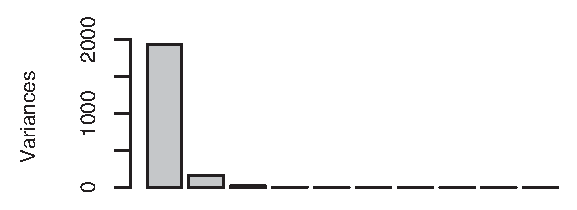
\includegraphics{img/screeplot}}
  \caption{A scree plot: the values of the principal components, from
    largest to smallest. Here, the largest component totally dominates
    the spectrum. But be careful: this result is spurious! (See
    text.)}
  \label{fig:screeplot}
\end{figure}

We see that the first eigenvalue entirely dominates the spectrum,
suggesting that the corresponding new variable is all that matters
(which of course would be great). To understand in more detail what is
going on, we look at the corresponding eigenvector. \index{eigenvectors} \index{vectors!eigenvectors} The
\texttt{print()} function is another overloaded function, which for
this particular data structure prints out the eigenvalues and
eigenvectors:

\begin{verbatim}
print( pc )

(some output omitted...)

                               PC1           PC2           PC3
fixed.acidity        -1.544402e-03 -9.163498e-03 -1.290026e-02
volatile.acidity     -1.690037e-04 -1.545470e-03 -9.288874e-04
citric.acid          -3.386506e-04  1.403069e-04 -1.258444e-03
residual.sugar       -4.732753e-02  1.494318e-02 -9.951917e-01
\end{verbatim}
\begin{verbatim}
chlorides            -9.757405e-05 -7.182998e-05 -7.849881e-05
free.sulfur.dioxide  -2.618770e-01  9.646854e-01  2.639318e-02
total.sulfur.dioxide -9.638576e-01 -2.627369e-01  4.278881e-02
density              -3.596983e-05 -1.836319e-05 -4.468979e-04
pH                   -3.384655e-06 -4.169856e-05  7.017342e-03
sulphates            -3.409028e-04 -3.611112e-04  2.142053e-03
alcohol               1.250375e-02  6.455196e-03  8.272268e-02

(some output omitted...)
\end{verbatim}

This is disturbing: if you look closely, you will notice that both the
first and the second eigenvector are dominated by the sulfur dioxide
concentration---and by a wide margin!  That does not seem right. I
don't understand much about wine, but I would not think that the
sulfur dioxide content is all that matters in the end.

Perhaps we were moving a little too fast. What do we actually know
about the data in the data set? Right: absolutely nothing! Time to
find out. One quick way to do so is to use the \texttt{summary()}
function on the \emph{original} data:\vspace*{9pt}

\begin{verbatim}
summary(wine)
fixed.acidity    volatile.acidity  citric.acid     residual.sugar  
Min.   : 3.800   Min.   :0.0800   Min.   :0.0000   Min.   : 0.600  
1st Qu.: 6.300   1st Qu.:0.2100   1st Qu.:0.2700   1st Qu.: 1.700  
Median : 6.800   Median :0.2600   Median :0.3200   Median : 5.200  
Mean   : 6.855   Mean   :0.2782   Mean   :0.3342   Mean   : 6.391  
3rd Qu.: 7.300   3rd Qu.:0.3200   3rd Qu.:0.3900   3rd Qu.: 9.900  
Max.   :14.200   Max.   :1.1000   Max.   :1.6600   Max.   :65.800  
  chlorides       free.sulfur.dioxide total.sulfur.dioxide    density     
Min.   :0.00900   Min.   :  2.00      Min.   :  9.0        Min.   :0.9871 
1st Qu.:0.03600   1st Qu.: 23.00      1st Qu.:108.0        1st Qu.:0.9917 
Median :0.04300   Median : 34.00      Median :134.0        Median :0.9937 
Mean   :0.04577   Mean   : 35.31      Mean   :138.4        Mean   :0.9940 
3rd Qu.:0.05000   3rd Qu.: 46.00      3rd Qu.:167.0        3rd Qu.:0.9961 
Max.   :0.34600   Max.   :289.00      Max.   :440.0        Max.   :1.0390 
      pH          sulphates         alcohol         quality     
Min.   :2.720   Min.   :0.2200   Min.   : 8.00   Min.   :3.000  
1st Qu.:3.090   1st Qu.:0.4100   1st Qu.: 9.50   1st Qu.:5.000  
Median :3.180   Median :0.4700   Median :10.40   Median :6.000  
Mean   :3.188   Mean   :0.4898   Mean   :10.51   Mean   :5.878  
3rd Qu.:3.280   3rd Qu.:0.5500   3rd Qu.:11.40   3rd Qu.:6.000  
Max.   :3.820   Max.   :1.0800   Max.   :14.20   Max.   :9.000  
\end{verbatim}

I am showing the output in its entire length to give you a sense of
the kind of output generated by R. If you look through this carefully,
you will notice that the two sulfur dioxide columns have values in the
tens to hundreds, whereas all other columns have values between $0.01$
and about $10.0$. This explains a lot: the two sulfur dioxide columns
dominate the eigenvalue spectrum simply because they were measured in
units that make the numerical values much larger than the other
quantities. As explained before, if this is the case, then we need to
\emph{scale} the input variables before performing the PCA. We can
achieve this by passing the \texttt{scale} option to the
\texttt{prcomp()} command, \index{prcomp() function} like
so:\vspace*{9pt}

\begin{verbatim}
pcx <- prcomp( wine, scale=TRUE )
\end{verbatim}

Before we examine the result of this operation, I'd like to point out
something else.  If you look really closely, you will notice that the
quality column is not what it claims to be. The description of the
original data set stated that quality was graded on a scale from 1 to
10.  But as we can see from the data summary, only grades between 3
and 9 have actually been assigned.  Worse, the first
quartile\vadjust{\pagebreak} is 5 and the third quartile is 6, which
means that at least half of all entries in the data set have a quality
ranking of either 5 or 6.  In other words, the actual range of qualities
is much narrower than we might have expected (given the original
description of the data) and is strongly dominated by the center.  This
makes sense (there are more mediocre wines than outstanding or terrible
ones), but it also makes this data set much less interesting because
whether a wine will be ranked 5 versus 6 during the sensory testing is
likely a toss-up.

We can use the \texttt{table()} function to see how often each quality
ranking occurs in the data set (remember that the dollar sign is used
to select a single column from the data frame):

\begin{verbatim}
table( wine$quality )

 3    4    5    6    7    8    9 
20  163 1457 2198  880  175    5 
\end{verbatim}\vspace*{-4pt}

As we suspected, the middling ranks totally dominate the distribution.
We might therefore want to change our goal and instead try to predict
the outliers, either good or bad, rather than spending too much effort
on the undifferentiated middle.

Returning to the results of the scaled PCA, we can look at the
spectrum of eigenvalues for the scaled version by using the
\texttt{summary()} function (again, overloaded!) on the return value
of \texttt{prcomp()}:

\begin{verbatim}
summary( pcx )
Importance of components:
                         PC1   PC2   PC3    PC4    PC5    PC6 
Standard deviation     1.829 1.259 1.171 1.0416 0.9876 0.9689 
Proportion of Variance 0.279 0.132 0.114 0.0904 0.0813 0.0782 
Cumulative Proportion  0.279 0.411 0.525 0.6157 0.6970 0.7752 
                         PC7    PC8    PC9    PC10   PC11   PC12
Standard deviation     0.8771 0.8508 0.7460 0.5856 0.5330 0.14307
Proportion of Variance 0.0641 0.0603 0.0464 0.0286 0.0237 0.00171
Cumulative Proportion  0.8393 0.8997 0.9460 0.9746 0.9983 1.00000
\end{verbatim}\vspace*{-4pt}

No single eigenvalue dominates now, and the first 5 (out of 12)
eigenvalues account for only 70 percent of the total variance.  That's
not encouraging---it doesn't seem that we can significantly reduce the
number of variables this way.

As a last attempt, we can create a biplot. \index{biplots, PCA} This, too, is very
simple; all we need to do is execute (see Figure \ref{fig:biplot})

\begin{verbatim}
biplot( pcx )
\end{verbatim}\vspace*{-4pt}

This is actually a fascinating graph! We see that three of the
original variables---alcohol content, sugar content, and density---
are parallel to the first principal component (the horizontal axis).
Moreover, alcohol content is aligned in the direction opposite to the
other two quantities.

\begin{figure}
  \centerline{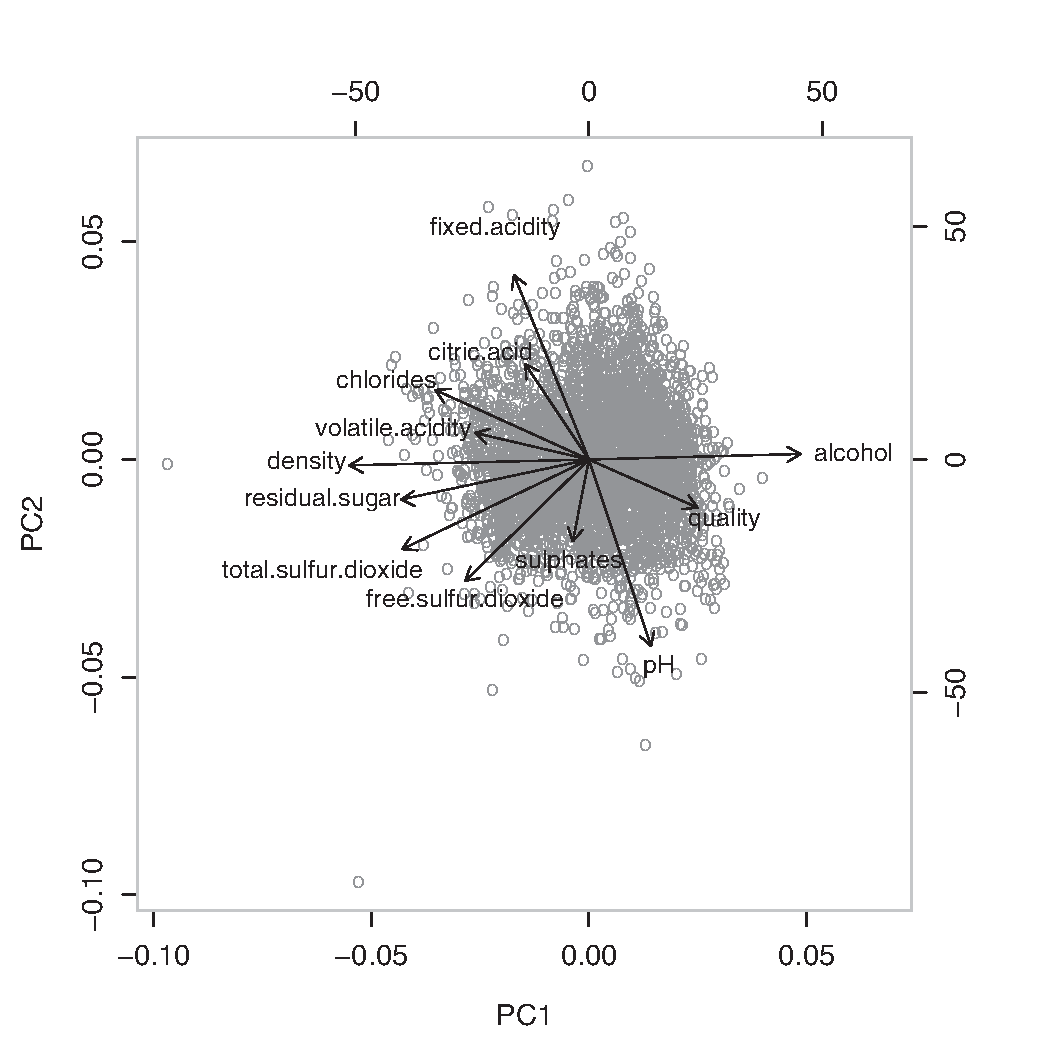
\includegraphics[width=\textwidth]{img/biplot}}
  \caption{A biplot: symbols correspond to the individual data points
    projected onto the plane spanned by the two largest principal
    components. Also shown are the original variables projected onto
    the same plane.}
  \label{fig:biplot}
\end{figure}

But this makes utmost sense. If you recall from chemistry class,
alcohol has a lower density than water, and sugar syrup has a
higher density. So the result of the PCA reminds us that density, sugar
concentration, and alcohol content are\vadjust{\pagebreak} not
independent: if you change one, the others will change accordingly.
And because these variables are parallel to the first principal
component, we can conclude that the overall density of the wine is an
important quantity.

The next set of variables that we can read off are the fixed acidity,
the citric acid concentration, and the pH value. Again, this makes
sense: the pH is a measure of the acidity of a solution (with higher
pH values indicating less acidity).  In other words, these three
variables are also at least partially redundant.

The odd one out, then, is the overall sulfur content, which is a
combination of sulfur dioxide and sulphate concentration.

And finally, it is interesting to see that the quality seems to be
determined primarily by the alcohol content and the acidity. This
suggests that the more alcoholic and the less sour the wine, the more
highly it is ranked---quite a reasonable conclusion!

We could have inferred all of this from the original description of
the data set, but I must say that I, for one, failed to see these
connections when initially scanning the list of columns. In this
sense, the PCA has been a tremendous help in interpreting and
understanding the content of the data set.

Finally, I'd like to reflect one more time on our use of R in this
example. This little application demonstrates both the power and the
shortcomings of R. On the one hand, R comes with many high-level,
powerful functions built in, often for quite advanced statistical
techniques (even an unusual and specialized graph like a biplot can be
created with a single command). On the other hand, the heavy reliance
on high-level functions with implicit behavior leads to opaque
programs that make it hard to understand exactly what is going on. For
example, such a critical question as deciding whether or not to
rescale the input data is handled as a rather obscure option to the
\texttt{prcomp()} command. In particular, the frequent use of
overloaded functions---which can exhibit widely differing
functionality depending on their input---makes it hard to predict the
precise outcome of an operation and makes discovering ways to perform
a specific action uncommonly difficult.

\index{dimensionality reduction!R statistical analysis package|)}
\index{R statistical analysis package|)}
\index{dimensionality reduction!principal component analysis (PCA)|)} 
\index{PCA (principal component analysis)!R statistical analysis package|)} 
\index{software!R statistical analysis package|)}

% ============================================================
\section{Further Reading}

\begin{itemize}
\item \cit{Introduction to Multivariate Analysis}{Chris Chatfield and
    Alexander Collins}{Chapman \& Hall/CRC}{1981}
  A bit dated but still one of the most practical, hands-on
  introductions to the mathematical theory of multivariate analysis.
  The section on PCA is particularly clear and practical but entirely
  skips computational issues and makes no mention of the SVD.

\item \cit{Principal Component Analysis}{I.\ T.\ Jolliffe}{2nd ed., 
    Springer}{2002}
  The definitive reference on principal component analysis. Not an
  easy read.

\item \cit{Multidimensional Scaling}{Trevor F.\ Cox and Michael A.\
    A.\ Cox}{Chapman \& Hall/CRC}{2001}
  The description of multidimensional scaling given in this chapter is
  merely a sketch---mostly, because I find it hard to imagine
  scenarios where this technique is truly useful. However, it has a
  lot of appeal and is fun to tinker with. Much more information,
  including some extensions, can be found in this book.

\item \cit{Introduction to Data Mining}{Pang-Ning Tan, Michael
    Steinbach, and Vipin Kumar}{Addison-Wesley}{2005}
  This is my favorite reference on data mining. The presentation is
  compact and more technical than in most other books on this topic.
\end{itemize}


\subsection{Linear Algebra}

\index{linear algebra}
\index{algebra!linear algebra}  

Linear algebra is a foundational topic. It is here that one encounters
for the first time abstract concepts such as spaces and mappings
treated as objects of interest in their own right. It takes time and
some real mental effort to get used to these notions, but one gains a
whole different perspective on things.

The material is also of immense practical value---particularly its
central result, which is the spectral decomposition theorem.  The
importance of this result cannot be overstated: it is used in
\emph{every} multi-dimensional problem in mathematics, science, and
engineering.

However, the material is abstract and unfamiliar, which makes it hard
for the beginner. Most introductory books on linear algebra try to
make the topic more palatable by emphasizing applications, but that
only serves to confuse matters even more, because it never becomes
clear why all that abstract machinery is needed when looking at
elementary examples. The abstract notions at the heart of linear
algebra are best appreciated, and most easily understood, when treated
in their own right.

The resources listed here are those I have found most helpful in this
regard.

\begin{itemize}
% \item XXX we need SOME elementary book here... XXX

\item \cit{Linear Algebra Done Right}{Sheldon Axler}{2nd ed.,
    Springer}{2004}
  The book lives up to its grandiose title. It treats linear algebra
  as an abstract theory of mappings but on a very accessible, advanced
  undergraduate level. Highly recommended but probably not as the first
  book on the topic.

\item \cit{Matrix Methods in Data Mining and Pattern Recognition}{Lars
    Eld\'en}{SIAM}{2007} 
  This short book is an introduction to linear algebra with a
  particular eye to applications in data mining. The pace is fast and
  probably requires at least some previous familiarity with the
  subject.

\item \cit{Understanding Complex Datasets: Data Mining with
    Matrix Decompositions}{David Skillicorn}{Chapman \& Hall/CRC}{2007}
  An advanced book, concentrating mostly on applications of the SVD
  and its variants.

\item \pcit{A Singularly Valuable Decomposition: The SVD of a
    Matrix}{Dan Kalman}{The College Mathematics Journal}{27}{1996}{2}
  This article, which can be found on the Web, is a nice introduction
  to the SVD. It's not for beginners, however.
\end{itemize}

\index{data analysis!dimensionality reduction|)}
\index{dimensionality reduction|)}

\clearpage

\thispagestyle{empty}

\cleardoublepage